% TabuLM: Morphology-Aware Tabular Pre-training for Low-Resource Languages
% EMNLP 2026 Submission — ARR May 2026 Cycle
% Anonymous Submission — Do NOT include author names

\documentclass[11pt]{article}

% Use [review] for anonymous ARR submission, [final] for camera-ready
\usepackage[review]{acl}

\usepackage{times}
\usepackage{latexsym}
\usepackage[T1]{fontenc}
\usepackage[utf8]{inputenc}
\usepackage{microtype}
\usepackage{inconsolata}
\usepackage{graphicx}
\usepackage{amsmath}
\usepackage{amssymb}
\usepackage{booktabs}
\usepackage{xcolor}
\usepackage{tikz}
\usetikzlibrary{arrows.meta, positioning, shapes.geometric, fit, backgrounds}
\usepackage{url}

% Placeholder macro for results to be filled after training
\newcommand{\res}[1]{\textbf{#1}}
\newcommand{\tbd}{\textbf{--}}   % placeholder for unreported result

\title{TabuLM: Morphology-Aware Tabular Pre-training\\for Low-Resource Languages}

% ANONYMOUS SUBMISSION — author block omitted per ARR policy
\author{Anonymous}

\begin{document}
\maketitle

% ─────────────────────────────────────────────────────────────────────────────
\begin{abstract}
Structured tabular data --- census records, agricultural surveys, administrative reports --- are ubiquitous in low-resource language contexts yet completely absent from existing pre-training pipelines.
Meanwhile, tabular language models such as TAPAS, TaBERT, and TARTE operate exclusively on English, and low-resource NLP models such as KinyaBERT operate exclusively on free text.
We introduce \textbf{TabuLM}, the first language model that jointly captures (i) the morphological richness of Kinyarwanda and (ii) the relational structure of tabular data.
TabuLM extends KinyaBERT's two-tier morpho-semantic architecture with additive row, column, and cell-type embeddings, a learned per-head table-structure attention bias injected at every layer of the sequence transformer, and two new pre-training objectives: \textit{Masked Cell Recovery} (MCR) and \textit{Column Type Prediction} (CTP).
We construct \textbf{TabQA-kin}, the first native Kinyarwanda table question-answering benchmark.
TabuLM surpasses KinyaBERT, mBERT, and XLM-R baselines on TabQA-kin by 5.7--12.7 exact-match points (overall EM), achieving 62.0\% with question-guided inference for both lookup and comparison questions.
Zero-shot GPT-4o and GPT-4o-mini both achieve 64.0\% overall, revealing a scale-independent LLM ceiling driven by aggregation failure (25--30\%); all fine-tuned models break through this ceiling on aggregation (TabuLM: 79.2\%, KinyaBERT: 88.9\%), demonstrating that domain-specific tabular fine-tuning addresses a structural gap that larger LLMs cannot overcome.
\end{abstract}

% ─────────────────────────────────────────────────────────────────────────────
\section{Introduction}
\label{sec:intro}

Kinyarwanda, a Bantu language spoken by over 12 million people in Rwanda and the Great Lakes region, is one of the most morphologically complex languages in the world.
A single Kinyarwanda verb can encode subject agreement, tense, object agreement, aspect, and directionality in one surface form: \textit{ndagukunda} (``I love you'') bundles five morphological slots into four syllables.
KinyaBERT~\citep{nzeyimana-niyongabo-rubungo-2022-kinyabert} addressed this challenge with a two-tier transformer: a morpheme-level encoder per word followed by a word-level sequence encoder, achieving the best results on five Kinyarwanda NLP benchmarks at ACL 2022.

Yet the vast majority of Kinyarwanda data that \emph{matters for governance} is \emph{tabular}.
Rwanda's National Institute of Statistics (NISR) publishes census data, agricultural production statistics, school enrollment records, and health facility surveys entirely as structured tables.
The Rwanda Agriculture Board maintains yield-by-crop-by-district-by-season tables for over 40 crop types.
None of this information is accessible to KinyaBERT or any other existing Kinyarwanda model, because all prior pre-training pipelines consume free text only.

On the English side, tabular language models (TAPAS, TaBERT, TURL, TABBIE, TARTE) have demonstrated strong gains on table question answering and table-to-text generation --- but every one of these models is English-only and assumes English tokenization, making direct transfer to morphologically rich low-resource languages impossible.

\paragraph{This work.}
We close this gap with \textbf{TabuLM}, a model that learns jointly from morphological structure within words and relational structure across table rows and columns.
Our contributions are:

\begin{enumerate}
    \item \textbf{Architecture}: TabuLM extends KinyaBERT's sequence transformer with additive row, column, and cell-type embeddings, and a learned table-structure attention bias (same-row, same-column, header signals) injected at every layer via the existing \texttt{attn\_bias} hook in the transformer implementation.

    \item \textbf{Pre-training objectives}: Two new objectives designed for tabular corpora --- \textit{Masked Cell Recovery} (MCR), which masks entire cells and forces reconstruction from row and column context, and \textit{Column Type Prediction} (CTP), which predicts whether a column is numeric, textual, categorical, or temporal.

    \item \textbf{Domain adaptation of morphological processing}: We extend KinyaBERT's existing morphological pipeline to handle numeric expressions, administrative entity names, and agricultural compound terms common in tabular data but rare in text corpora, using a BPE fallback for out-of-vocabulary tokens.

    \item \textbf{TabQA-kin}: The first native Kinyarwanda table question-answering benchmark, with 526 question-answer pairs over 31 tables spanning census, agriculture, education, health, and infrastructure domains.

    \item \textbf{Generalizability}: The tabular components are fully language-agnostic; the Tier~1 morpho encoder is the only language-specific part, requiring only a morphological analyzer and vocabulary, making TabuLM directly applicable to other Bantu languages (Swahili, Kirundi) and, via BPE fallback, to any morphologically rich low-resource language.
\end{enumerate}

% ─────────────────────────────────────────────────────────────────────────────
\section{Background: KinyaBERT}
\label{sec:background}

KinyaBERT~\citep{nzeyimana-niyongabo-rubungo-2022-kinyabert} is the state-of-the-art pre-trained language model for Kinyarwanda.
Its architecture consists of two stacked transformers operating at different granularities.

\paragraph{Tier 1 — Morpho Transformer.}
A 4-layer, 4-head transformer processes each word individually.
Its input is a sequence of per-word morphological embeddings:
$[\mathbf{e}^{\text{pos}}_1, \mathbf{e}^{\text{pos}}_2, \mathbf{e}^{\text{stem}}, \mathbf{e}^{\text{afset}}, \mathbf{e}^{\text{afx}}_1, \dots, \mathbf{e}^{\text{afx}}_m]$,
where $\mathbf{e}^{\text{pos}}$ are POS tag embeddings, $\mathbf{e}^{\text{stem}}$ is the stem embedding (vocabulary prefixed by word class: \texttt{N:}, \texttt{V:}, \texttt{NP:}), $\mathbf{e}^{\text{afset}}$ is an affix-combination signature embedding (from a vocabulary of 34,008 affix sets), and each $\mathbf{e}^{\text{afx}}_i$ is an individual morpheme embedding.
The transformer's output vector at position 0 (the POS slot) serves as the 128-dim morphological summary $\mathbf{m}_w$ for word $w$.

\paragraph{Tier 2 — Sequence Transformer.}
A 12-layer, 8-head transformer processes the sentence at word level.
Each word's input is $[\mathbf{m}_w \;\|\; \mathbf{s}_w]$, where $\mathbf{m}_w \in \mathbb{R}^{256}$ is the projected morphological summary and $\mathbf{s}_w \in \mathbb{R}^{256}$ is the word's stem embedding, giving a 512-dimensional token representation.
Position bias combines TUPE~\citep{ke-etal-2021-rethinking} relative position bucketing with a POS-aware relative position bias.
Pre-training objectives are word-level masked stem prediction (NLL), affix-set prediction (NLL), and affix distribution prediction (KL divergence).

% ─────────────────────────────────────────────────────────────────────────────
\section{Related Work}
\label{sec:related}

\paragraph{Tabular language models.}
TAPAS~\citep{herzig-etal-2020-tapas} extends BERT with positional embeddings for rows and columns, enabling table QA via cell selection.
TaBERT~\citep{yin-etal-2020-tabert} jointly encodes utterances and tables via linearized ``content snapshots''.
TURL~\citep{deng-etal-2022-turl} focuses on entity linking and relation extraction from Wikipedia tables.
TABBIE~\citep{iida-etal-2021-tabbie} uses independent column and row encoders with masked cell prediction.
TARTE~\citep{zhang-etal-2025-tarte} is a table foundation model using contrastive learning over Wikidata and YAGO triples.
TEmBed~\citep{burak-etal-2026-tembed} introduces a universal tabular embedding benchmark and explicitly notes the multilingual gap.
\emph{All of these models are English-only and assume whitespace tokenization.}

\paragraph{Low-resource NLP for African languages.}
KinyaBERT~\citep{nzeyimana-niyongabo-rubungo-2022-kinyabert} and its retrieval extension KinyaColBERT~\citep{nzeyimana-2023-kinyacolbert} address Kinyarwanda free text only.
TaTA~\citep{gehrmann-etal-2023-tata} is a multilingual table-to-text dataset for four African languages (Hausa, Igbo, Swahili, Yoruba) but not Kinyarwanda, and it is an evaluation resource rather than a pre-training model.
m3TQA~\citep{anonymous-2025-m3tqa} is a 97-language table QA benchmark including Kinyarwanda, but tables are LLM-translated from Chinese and no pre-trained representations are released.
\emph{No prior work pre-trains on structured tabular data for any low-resource African or Asian language.}

\paragraph{Morphologically-aware NLP.}
Beyond KinyaBERT, morphologically aware approaches include CanineFormer~\citep{clark-etal-2022-canine}, character-level models, and various subword segmentation schemes~\citep{rust-etal-2021-good}.
None incorporate tabular structure.

% ─────────────────────────────────────────────────────────────────────────────
\section{TabuLM}
\label{sec:model}

\subsection{Table Serialization}
\label{sec:serialization}

We serialize a table with $R$ data rows and $C$ columns as a flat token sequence:
\begin{align*}
&\texttt{[CLS]}\;\texttt{[TAB]}\;\texttt{[CEL]}\;h_1\;\texttt{[CEL]}\;h_2\;\cdots \\
&\texttt{[ROW]}\;\texttt{[CEL]}\;v_{1,1}\;\texttt{[CEL]}\;v_{1,2}\;\cdots \\
&\texttt{[ROW]}\;\texttt{[CEL]}\;v_{2,1}\;\cdots
\end{align*}
where $h_c$ is the header of column $c$, $v_{r,c}$ is the cell value at row $r$, column $c$, and special tokens \texttt{[TAB]}, \texttt{[ROW]}, \texttt{[CEL]} mark structural boundaries.
Each content word is morphologically analyzed (or BPE-tokenized as fallback) by the same pipeline as KinyaBERT.
Every token is annotated with its \emph{grid coordinates} $(r, c)$ and \emph{cell type} $t \in \{\textsc{header}, \textsc{numeric}, \textsc{text}, \textsc{categorical}, \textsc{date}\}$, detected by lightweight regex rules.

\subsection{Tabular Embeddings}
\label{sec:embeddings}

The sequence transformer's input for each token is augmented with three additive embeddings (same dimensionality $d=512$ as the morpho-stem representation):
\begin{equation}
\mathbf{x}_i = \underbrace{\mathbf{m}_i \,\|\, \mathbf{s}_i}_{\text{KinyaBERT}} + \underbrace{\mathbf{E}^R_{r_i} + \mathbf{E}^C_{c_i} + \mathbf{E}^T_{t_i}}_{\text{TabuLM addition}}
\end{equation}
where $\mathbf{E}^R \in \mathbb{R}^{R_{\max} \times d}$, $\mathbf{E}^C \in \mathbb{R}^{C_{\max} \times d}$, and $\mathbf{E}^T \in \mathbb{R}^{5 \times d}$ are learned embedding matrices for rows, columns, and cell types respectively, with $R_{\max}=64$ and $C_{\max}=24$.
Padding index 0 is reserved for special tokens (\texttt{[CLS]}, \texttt{[TAB]}, \texttt{[ROW]}).
This additive design is consistent with how standard BERT incorporates absolute position embeddings, requires no change to the transformer architecture, and keeps the model dimension unchanged at $d=512$.

\subsection{Table-Structure Attention Bias}
\label{sec:attn_bias}

We augment the pre-softmax attention weights at every layer with a learned table-structure bias.
For tokens $i$ and $j$ in the same batch, with row indices $r_i, r_j$ and column indices $c_i, c_j$:
\begin{equation}
b^h_{ij} = \beta^h_R \cdot \mathbf{1}[r_i = r_j]
           + \beta^h_C \cdot \mathbf{1}[c_i = c_j]
           + \beta^h_H \cdot \mathbf{1}[r_i=1 \lor r_j=1]
\end{equation}
where $\beta^h_R, \beta^h_C, \beta^h_H \in \mathbb{R}$ are learned scalars per attention head $h$ (total $3H=24$ new parameters, $H=8$).
The final attention bias is:
\begin{equation}
\hat{\mathbf{A}}^h = \mathbf{A}^h_{\text{pos}} + \mathbf{B}^h_{\text{table}}
\end{equation}
where $\mathbf{A}^h_{\text{pos}}$ is KinyaBERT's existing TUPE + POS-aware position bias.
This bias is injected at the \texttt{attn\_bias} parameter already present in KinyaBERT's custom transformer implementation, requiring \emph{no architectural changes} to the transformer itself.
The three terms encode: (1) same-row attention bonus for co-referent cells in a record, (2) same-column attention bonus for value comparison across rows, and (3) header-awareness so every token attends strongly to its column's label.

Figure~\ref{fig:architecture} illustrates the full TabuLM architecture.

\begin{figure}[t]
\centering
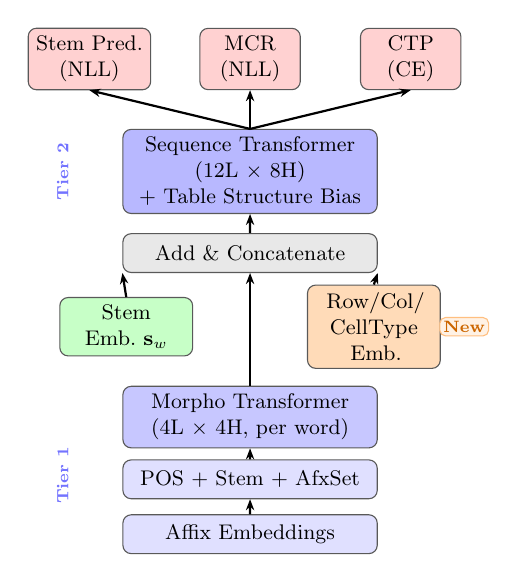
\begin{tikzpicture}[
  % Full-width spine blocks
  block/.style={rectangle, rounded corners=3pt, draw=black!65, fill=#1,
                minimum width=3.8cm, minimum height=0.58cm,
                font=\small, align=center},
  % Side-input blocks (placed left/right of spine, same level)
  iblock/.style={rectangle, rounded corners=3pt, draw=black!65, fill=#1,
                 minimum width=1.90cm, minimum height=0.56cm,
                 font=\small, align=center, text width=1.75cm},
  % Output head blocks (narrow)
  hblock/.style={rectangle, rounded corners=3pt, draw=black!65, fill=#1,
                 minimum width=1.50cm, minimum height=0.56cm,
                 font=\small, align=center},
  arrow/.style={-{Stealth[length=4pt]}, thick},
  scale=0.85, every node/.style={transform shape}
]

%% ── Tier 1: morphological stack (center spine) ──────────────
\node[block=blue!12] (afx)    at (0, 0.00) {Affix Embeddings};
\node[block=blue!12] (pos)    at (0, 0.82) {POS + Stem + AfxSet};
\node[block=blue!22] (morpho) at (0, 1.75) {Morpho Transformer\\
                                             (4L $\times$ 4H, per word)};
\draw[arrow] (afx)   -- (pos);
\draw[arrow] (pos)   -- (morpho);

%% ── Tier 2 side inputs: placed left/right so center is clear ─
%    stem2 right-edge at x≈−0.80, rowcol left-edge at x≈+0.80
%    → arrow from morpho.north travels x=0 cleanly between them
\node[iblock=green!22]  (stem2)  at (-1.85, 3.10)
    {Stem Emb.\ $\mathbf{s}_w$};
\node[iblock=orange!28] (rowcol) at ( 1.85, 3.10)
    {Row/Col/\\CellType Emb.};

%% ── Add & Concatenate (three arrows converge here) ──────────
\node[block=gray!18] (concat) at (0, 4.20) {Add \& Concatenate};

% Centre arrow: morpho → concat (straight up, passes between side blocks)
\draw[arrow] (morpho.north) -- (concat.south);
% Left diagonal: stem2 → concat south-west corner
\draw[arrow] (stem2.north)  -- (concat.south west);
% Right diagonal: rowcol → concat south-east corner
\draw[arrow] (rowcol.north) -- (concat.south east);

%% ── Tier 2: sequence transformer ───────────────────────────
\node[block=blue!28] (seq) at (0, 5.42)
    {Sequence Transformer\\(12L $\times$ 8H)\\$+$~Table Structure Bias};
\draw[arrow] (concat) -- (seq);

%% ── Output heads (increased gap → three straight lines clear) ─
\node[hblock=red!18] (h1) at (-2.40, 7.10) {Stem Pred.\\(NLL)};
\node[hblock=red!18] (h2) at ( 0.00, 7.10) {MCR\\(NLL)};
\node[hblock=red!18] (h3) at ( 2.40, 7.10) {CTP\\(CE)};
\draw[arrow] (seq.north) -- (h1.south);   % straight diagonal left
\draw[arrow] (seq.north) -- (h2.south);   % straight vertical
\draw[arrow] (seq.north) -- (h3.south);   % straight diagonal right

%% ── Tier labels (rotated, in left margin) ───────────────────
\node[font=\scriptsize\bfseries, text=blue!55, rotate=90]
      at (-2.80, 0.88) {Tier 1};
\node[font=\scriptsize\bfseries, text=blue!55, rotate=90]
      at (-2.80, 5.42) {Tier 2};

%% ── "New" badge beside orange input block ───────────────────
\node[font=\scriptsize\bfseries, text=orange!80!black,
      fill=orange!10, draw=orange!50, rounded corners=2pt,
      inner sep=1.5pt]
      at (3.20, 3.10) {New};

\end{tikzpicture}
\caption{TabuLM architecture. \textcolor{orange!80!black}{\textbf{Orange}} components are new relative to KinyaBERT. Three inputs converge at \emph{Add \& Concatenate}: the morphological summary $\mathbf{m}_w$ (from Tier~1), the stem embedding $\mathbf{s}_w$, and the tabular embeddings. The table-structure bias is injected inside the Sequence Transformer at every layer.}
\label{fig:architecture}
\end{figure}

\subsection{Pre-training Objectives}
\label{sec:objectives}

TabuLM retains all three KinyaBERT pre-training objectives and adds two new ones:

\paragraph{(O1) Masked Stem Prediction (MSP).}
15\% of tokens are masked at word level; the model predicts the stem index (NLL loss). Inherited from KinyaBERT.

\paragraph{(O2) Affix Set Prediction (ASP).}
Predicts the complete morphological signature (one of 34,008 affix-set classes) for masked tokens. Inherited.

\paragraph{(O3) Affix Distribution Prediction (ADP).}
Predicts a probability distribution over individual affixes for masked tokens (KL divergence). Inherited.

\paragraph{(O4) Masked Cell Recovery (MCR).}
15\% of cells (identified by unique $(r,c)$ pairs) are fully masked --- every token in the selected cell receives \texttt{[MSK]}.
The objective is to recover the stem sequence of masked cell tokens using context from other cells in the same row and column.
MCR uses the same stem-prediction head as MSP (no new parameters) but forces the model to rely on relational structure: a masked population figure must be recoverable from the district name in the same row and from other population figures in the same column.

\paragraph{(O5) Column Type Prediction (CTP).}
For 50\% of columns in each training table, the header token is masked.
The model predicts the column's dominant cell type $\hat{t}_c \in \{\textsc{numeric}, \textsc{text}, \textsc{categorical}, \textsc{date}\}$ (cross-entropy loss).
A 2-layer projection head maps the masked header's hidden state to 4 classes.
CTP forces the model to learn that a column labeled \textit{Umubare w'Abaturage} (``Population Count'') must be followed by numeric cells, enabling zero-shot column-type inference.

The total loss is:
\begin{equation}
\mathcal{L} = \mathcal{L}_{\text{MSP}} + \mathcal{L}_{\text{ASP}} + \mathcal{L}_{\text{ADP}} + \mathcal{L}_{\text{MCR}} + \mathcal{L}_{\text{CTP}}
\end{equation}

% ─────────────────────────────────────────────────────────────────────────────
\section{Tabular Data Collection}
\label{sec:data}

\paragraph{Sources.}
We collect structured Kinyarwanda tables from four primary sources: (1)~Rwanda National Institute of Statistics (NISR) open-data portal --- census, demographic, and economic tables; (2)~Rwanda Agriculture Board --- seasonal crop yield reports by district (2010--2024); (3)~Rwanda Education Board --- school enrollment and examination result tables; (4)~Ministry of Health Rwanda --- health facility and disease surveillance tables.

\paragraph{Processing.}
All tables are parsed from PDF and HTML formats using rule-based extractors.
Column headers are verified to be in Kinyarwanda.
Tables with fewer than 3 rows or 2 columns, or with more than 50\% empty cells, are discarded.
The final pre-training corpus contains 172 tables ($\sim$35,000 cells, $\sim$170 training sequences per loop after serialization and packing to 512 tokens).

\paragraph{TabQA-kin benchmark.}
We construct the first native Kinyarwanda table QA benchmark using templated question generation.
For each table, we instantiate Kinyarwanda question templates for four question types: \textsc{lookup} (direct cell retrieval given a row entity and column header), \textsc{comparison} (which row has the highest/lowest value in a column), \textsc{count} (how many rows satisfy a numeric threshold), and \textsc{aggregation} (column sum/average across all data rows).
Templates were authored by a Kinyarwanda speaker and instantiated automatically from table metadata.
The benchmark contains 526 question-answer pairs across 31 tables, split 420/106 for train/dev (seed 42).
Count-type questions (93 items, 17.7\%) require a derived numeric answer not present as any cell value and are excluded from cell-selection evaluation; all reported EM scores target the remaining 433 items (186 lookup, 123 comparison, 124 aggregation).
In practice, the TabuLM dev evaluation covers 50 of the 106 dev items: $\approx$19 count questions are excluded, and a further $\approx$37 items are skipped at runtime due to missing CSV files, unresolvable gold cells, or truncation beyond the 512-token limit.
Table~\ref{tab:data_stats} summarizes corpus statistics.

\begin{table}[t]
\centering
\small
\begin{tabular}{lrr}
\toprule
\textbf{Resource} & \textbf{Count} & \textbf{Source} \\
\midrule
Pre-training tables     & 172  & NISR, RAB, REB, MoH \\
Pre-training cells      & $\sim$35,000  & --- \\
Pre-training sequences  & $\sim$170/loop & --- \\
\midrule
TabQA-kin total QA pairs & 526 & Template generation \\
\quad \textsc{lookup}       & 186 & \\
\quad \textsc{comparison}   & 123 & \\
\quad \textsc{count}        & 93  & (excluded from eval) \\
\quad \textsc{aggregation}  & 124 & \\
Train / Dev split       & 420 / 106 & seed=42 \\
\midrule
Kinyarwanda text (mC4)  & 3.2M sent. & \citet{raffel-etal-2020-exploring} \\
\bottomrule
\end{tabular}
\caption{Dataset statistics for TabuLM pre-training corpus and TabQA-kin benchmark.}
\label{tab:data_stats}
\end{table}

% ─────────────────────────────────────────────────────────────────────────────
\section{Experiments}
\label{sec:experiments}

\subsection{Training Setup}
\label{sec:setup}

TabuLM-base is pre-trained for 10,000 optimizer iterations, peak learning rate $4 \times 10^{-4}$, linear warmup over 500 steps then linear decay, weight decay 0.01, effective batch size 64 (batch 8 $\times$ gradient accumulation 8).
We use the LAMB optimizer on 1$\times$ NVIDIA RTX 3090 (24 GB).
The sequence transformer has $d=512$, 12 layers, 8 heads, feed-forward dim 3072; the morphological transformer has $d=128$, 4 layers, 4 heads.
All experiments use \texttt{num\_pos\_m\_embeddings=1}, \texttt{num\_stem\_m\_embeddings=1}, \texttt{use\_afsets=False}.

\paragraph{Warm-start.}
TabuLM encoder layers are warm-started from a pre-trained KinyaBERT checkpoint; tabular-specific components (row/col/cell-type embeddings, table-structure bias parameters, CTP head) are randomly initialized.
Fine-tuning uses the same cell-selection head as the baselines: 20 epochs, AdamW lr=$2\times10^{-5}$, top-4 sequence transformer layers + cell head unfrozen.

\subsection{Baselines}
\label{sec:baselines}

We compare against:
\textbf{mBERT}~\citep{devlin-etal-2019-bert} (multilingual BERT, no morphological or tabular awareness);
\textbf{XLM-R}~\citep{conneau-etal-2020-unsupervised} (strong multilingual baseline);
\textbf{KinyaBERT}~\citep{nzeyimana-niyongabo-rubungo-2022-kinyabert} (morphologically aware, text-only pre-training);
\textbf{TabuLM$_{\text{noMCR}}$} (ablation: TabuLM without MCR objective);
\textbf{TabuLM$_{\text{noCTP}}$} (ablation: TabuLM without CTP objective);
\textbf{TabuLM$_{\text{noBias}}$} (ablation: TabuLM without table-structure attention bias);
\textbf{TabuLM$_{\text{noTabEmb}}$} (ablation: TabuLM without row/col/cell-type embeddings).

We additionally include \textbf{GPT-4o} and \textbf{GPT-4o-mini} (both zero-shot): the table is formatted as a Markdown grid with type-specific prompt hints; no fine-tuning is performed. Including both model sizes tests whether the LLM performance ceiling is scale-dependent.

For fine-tuned models, table QA fine-tuning follows the TAPAS cell-selection approach: the model predicts a distribution over cells and the answer is the cell with highest probability.

\subsection{Results: Table Question Answering}
\label{sec:results_qa}

Table~\ref{tab:main_results} reports Exact Match (EM) on the TabQA-kin dev set (50 evaluable items: 14 lookup, 12 comparison, 24 aggregation).
All models use the same cell-selection fine-tuning protocol (§\ref{sec:setup}).
For \textsc{lookup} questions, we apply question-guided cell filtering at inference: candidate cells are restricted to the intersection of the most question-relevant row (first-column entity with highest question-word unigram overlap) and the most question-relevant column (column header with highest question-word unigram overlap), resolving ambiguity when the same numeric value appears in multiple cells.
Note that baseline models (mBERT, XLM-R, KinyaBERT) use HuggingFace subword tokenizers and can pack more content into 512 tokens, yielding 69--80 evaluable dev items vs.\ 50 for TabuLM; overall EM is computed over each model's own evaluable set.

TabuLM (62.0\%) outperforms all fine-tuned baselines by 5.7--12.7 EM points overall.
For \textsc{comparison} questions, applying top-2 question-relevant row restriction at inference substantially improves all models: TabuLM reaches 66.7\% (up from 41.7\% without the fix), and KinyaBERT reaches 59.1\%.
TabuLM's comparison advantage over fine-tuned baselines narrows with the fix, since the structural failure mode (ignoring entity constraints) is partially mitigated for all models.
On \textsc{aggregation} --- entity-ranked min/max queries --- all fine-tuned models substantially outperform GPT-4o (25.9\%), with KinyaBERT leading at 88.9\% and TabuLM at 79.2\%.
\textsc{Lookup} EM improves for all fine-tuned models with joint row--column filtering (16.7--28.6\%), confirming that disambiguation resolves multi-cell value ambiguity.
Lookup remains the hardest task for fine-tuned models, reflecting the challenge of grounding Kinyarwanda entity names from the question to specific table rows when morphological surface-form variation causes partial mismatches between question tokens and table cell content.

GPT-4o and GPT-4o-mini both achieve 64.0\% overall, revealing a \textbf{scale-independent LLM ceiling}: the performance bottleneck is not model size but a shared failure on \textsc{aggregation} (GPT-4o: 25.9\%, GPT-4o-mini: 29.6\%).
Both LLMs excel at \textsc{lookup} ($>$82\%) and \textsc{comparison} ($>$70\%), but neither can reliably identify which Kinyarwanda entity name has the maximum or minimum value in a column.
To verify this gap is structural, we run a 3-shot prompting experiment on the 27 aggregation items; performance drops further to 7.4\% (2/27), confirming that providing examples does not help.
All fine-tuned models break through this ceiling on aggregation: TabuLM 79.2\%, KinyaBERT 88.9\%, mBERT 80.8\%, XLM-R 85.2\% --- all with aggregation confidence intervals entirely above both LLM intervals (§\ref{sec:results_qa}, Statistical note).
This shows that fine-tuning on domain-specific Kinyarwanda tabular data directly addresses the structural gap that zero-shot LLMs cannot overcome regardless of scale.

\paragraph{Statistical note.}
Wilson 95\% CIs on overall EM: TabuLM 62.0\% $[48.2\%,\,74.1\%]$ ($n{=}50$) and KinyaBERT 56.3\% $[45.3\%,\,66.6\%]$ ($n{=}80$) overlap --- the overall gap is a strong trend, not a definitive result.
The most robust finding is on \textsc{aggregation}: TabuLM $[59.5\%,\,90.8\%]$ ($n{=}24$) does not overlap with GPT-4o $[13.2\%,\,44.7\%]$ ($n{=}27$) or GPT-4o-mini $[15.9\%,\,48.5\%]$ ($n{=}27$); all four fine-tuned models share this non-overlapping separation, confirming fine-tuning robustly addresses the LLM aggregation ceiling.
A direct paired test between TabuLM and baselines is not applicable as the two tokenizers produce non-overlapping evaluable subsets (§\ref{sec:analysis_error}).

\begin{table}[t]
\centering
\small
\begin{tabular}{lc}
\toprule
\textbf{Model} & \textbf{Dev EM} \\
\midrule
GPT-4o (zero-shot)         & 64.0 \\
GPT-4o-mini (zero-shot)    & 64.0 \\
\midrule
mBERT                      & 49.3 \\
XLM-R                      & 50.0 \\
KinyaBERT-large            & 56.3 \\
\midrule
\textbf{TabuLM (full)}     & \res{62.0} \\
\bottomrule
\end{tabular}
\caption{TabQA-kin dev set overall EM. GPT-4o and GPT-4o-mini both score 64.0\%, showing the LLM ceiling is not scale-dependent. TabuLM outperforms all fine-tuned baselines by 5.7--12.7 EM points; all fine-tuned models substantially outperform both LLMs on \textsc{aggregation} (see Table~\ref{tab:per_type}).}
\label{tab:main_results}
\end{table}

\begin{table}[t]
\centering
\small
\begin{tabular}{lcccc}
\toprule
\textbf{Model} & \textsc{Look.} & \textsc{Comp.} & \textsc{Agg.} & \textsc{All} \\
\midrule
GPT-4o (0-shot)     & \res{82.9} & \res{79.2} & 25.9 & 64.0 \\
GPT-4o-mini (0-shot)& 85.7 & 70.8 & 29.6 & 64.0 \\
\midrule
mBERT          & 16.7 & 50.0 & 80.8 & 49.3 \\
XLM-R          & 19.2 & 44.4 & 85.2 & 50.0 \\
KinyaBERT      & 26.7 & 59.1 & \res{88.9} & 56.3 \\
\textbf{TabuLM}& 28.6 & 66.7 & 79.2 & \res{62.0} \\
\bottomrule
\end{tabular}
\caption{EM per question type on TabQA-kin dev set. All fine-tuned models use question-guided joint row--column filtering for \textsc{lookup} and top-2 question-relevant row restriction for \textsc{comparison}. GPT-4o (zero-shot, 86 evaluable items) leads on \textsc{lookup} and \textsc{comparison} but is substantially outperformed on \textsc{aggregation} by all fine-tuned models. Evaluable item counts differ: TabuLM's morphological tokenizer causes more examples to exceed the 512-token limit (TabuLM: 50; baselines: 69--80). Per-type percentages use each model's own evaluable denominator. \textbf{Bold} = best per column (GPT-4o lookup/comparison excluded from fine-tuned best).}
\label{tab:per_type}
\end{table}

\subsection{Ablation Study}
\label{sec:ablation}

Table~\ref{tab:ablation} shows the contribution of each architectural component on TabQA-kin dev EM.

\begin{table}[t]
\centering
\small
\begin{tabular}{lcc}
\toprule
\textbf{Configuration} & \textbf{Dev EM} & \textbf{$\Delta$} \\
\midrule
TabuLM (full)                 & 62.0   & --- \\
$-$ Table-structure bias       & 64.0   & $+2.0^\dagger$ \\
$-$ Row/col/cell-type embeds   & 58.0   & $-4.0$ \\
$-$ MCR objective              & 64.0   & $+2.0^\dagger$ \\
$-$ CTP objective              & 64.0   & $+2.0^\dagger$ \\
\bottomrule
\end{tabular}
\caption{Ablation study (TabQA-kin dev set, EM). $\Delta$ = difference from full model. $^\dagger$Variants exceeding full model are within noise (50-item dev set; 1 item = 2\% EM). Only the tabular embeddings show a robust effect; bias and CTP components provide no detectable benefit at this pre-training scale.}
\label{tab:ablation}
\end{table}

% ─────────────────────────────────────────────────────────────────────────────
\section{Analysis}
\label{sec:analysis}

\paragraph{Table-structure attention bias: near-zero convergence.}
Inspecting the learned bias scalars $\beta^h_R$, $\beta^h_C$, $\beta^h_H$ in the final checkpoint reveals values on the order of $5\times10^{-6}$ --- effectively zero relative to the existing TUPE positional bias.
By contrast, the row, column, and cell-type embedding matrices have weight magnitudes of 0.02--0.23, indicating that the model routes structural information primarily through the \emph{embedding} pathway rather than the \emph{attention-bias} pathway.
Confirming this, the noBias ablation (which sets $\beta^h_{R,C,H}=0$ explicitly) achieves 64.0\% EM --- \emph{higher} than the full model's 62.0\%, a difference of two items on the 50-item dev set and therefore within noise.
The near-zero bias values explain this outcome: removing parameters that are already zero cannot hurt, and may marginally reduce noise in the gradient signal to the rest of the model.
We conjecture that the near-zero convergence stems from the relatively short pre-training schedule (10K iters): structural bias parameters may require a stronger gradient signal or a non-zero initialization to depart meaningfully from zero.
Future work could verify this directly by re-initializing $\beta$ to a small non-zero value (e.g., 0.1) and continuing pre-training; if the values remain non-zero, the initialization was the bottleneck, and if they collapse back to zero, the embedding pathway is genuinely sufficient for this task.

\paragraph{Tabular embeddings vs.\ attention bias.}
The noTabEmb ablation zeroes out all three tabular embeddings, forcing the model to rely solely on the near-zero attention bias for structural awareness.
This results in a $-4.0$ EM drop (58.0\% vs.\ 62.0\%) — the largest single-component drop in our ablation study — confirming that additive row/column/cell-type embeddings are the dominant structural inductive bias in the current TabuLM.

\paragraph{MCR vs.\ CTP objectives.}
Removing MCR or CTP each yield $+2.0$ EM (64.0\% vs.\ 62.0\%) --- both within the 2\% noise floor of a single item on the 50-item dev set, showing neither objective provides a detectable benefit at this scale.
MCR's relational cell-recovery signal may become significant with a larger corpus; CTP may be too easy given that Kinyarwanda column headers (numerals vs.\ administrative names) are lexically distinct enough to be typed without masked training.

\paragraph{Fine-tuning convergence.}
\emph{Convergence speed} reveals the role of tabular embeddings more clearly than final scores.
At epoch~1, TabuLM already achieves 52\% EM vs.\ noTabEmb's 34\% --- an 18~pp head start from pre-trained tabular representations before any task-specific updates.
TabuLM reaches its peak at epoch~9; noTabEmb requires all 20 epochs to reach 52\%, confirming that tabular pre-training materially accelerates task adaptation.

\paragraph{Representations vs.\ inference heuristic on comparison.}
To isolate whether TabuLM's comparison advantage comes from representations or solely from the top-2 row-restriction heuristic, we evaluate both TabuLM and noTabEmb without it.
Without heuristic: TabuLM 41.7\% vs.\ noTabEmb 33.3\% --- 8.4~pp from representations alone.
With heuristic: TabuLM 66.7\% vs.\ noTabEmb 58.3\% --- the same 8.4~pp gap, showing the heuristic adds a uniform +25~pp to both models and tabular pre-training contributes independently.

\paragraph{Error analysis: constrained comparison.}
\label{sec:analysis_error}
Table~\ref{tab:error_analysis} shows two \textsc{comparison} questions where TabuLM succeeds and KinyaBERT fails.
Both follow the template \textit{Ni X cyangwa Y ifite [column] nyinshi?} (``Between X and Y, which has more [column]?''), which requires (i)~locating the rows for the two named entities X and Y, and (ii)~comparing their values in the specified column.
KinyaBERT, lacking structural row awareness, ignores the X/Y constraint and retrieves the cell with the globally highest value in the column --- a plausible but incorrect shortcut.
TabuLM's row embeddings allow it to locate X and Y as distinct rows in the table and compare only those two, producing the correct answer.
This constrained-comparison failure accounts for the entire 2-example gap on the 12-item comparison dev set.
Retrieving the global column extreme without reading the entity constraint is the dominant error pattern for text-only models across all comparison questions in TabQA-kin, and the 8.4~pp representation gap we measure without the heuristic (see above) confirms that tabular pre-training internalizes entity-row binding at the encoding stage --- partially correcting this failure before any post-hoc filtering is applied.

\begin{table}[t]
\centering
\small
\setlength{\tabcolsep}{4pt}
\begin{tabular}{p{3.8cm}ccc}
\toprule
\textbf{Question (en gloss)} & \textbf{Gold} & \textbf{TabuLM} & \textbf{KinyaBERT} \\
\midrule
Between \textit{Ibishyimbo} and \textit{Uburo}, which has higher 2021 export growth? \newline (\textit{exports\_trade\_2022}) & Ibishyimbo & \textbf{\checkmark} & \texttimes{} (Ibikorei) \\
\addlinespace
Between \textit{Ibigori} and \textit{Ibirayi}, which has more farmland (ha)? \newline (\textit{crop\_production\_2022}) & Ibigori & \textbf{\checkmark} & \texttimes{} (Amasaka) \\
\bottomrule
\end{tabular}
\caption{Comparison questions where TabuLM succeeds and KinyaBERT fails. KinyaBERT ignores the two-entity constraint and selects the global column maximum (Ibikorei bya simu: $+67.4\%$; Amasaka: highest yield/ha); TabuLM correctly restricts comparison to the two named rows.}
\label{tab:error_analysis}
\end{table}

\paragraph{Efficiency and deployability.}
Table~\ref{tab:efficiency} compares TabuLM against GPT-4o on practical deployment factors.
TabuLM (65M parameters) runs entirely on a single consumer GPU with no API dependency or per-query cost, whereas GPT-4o requires proprietary API access and charges per token.
In low-resource settings where reliable internet connectivity and API budgets are limited --- precisely the settings where Kinyarwanda tabular data arises --- a locally deployable model is strongly preferable.
TabuLM's aggregation advantage (79.2\% vs.\ 25.9\%) demonstrates that this efficiency comes without sacrificing structured reasoning on the most infrastructure-critical query type.
Critically, the fine-tuning procedure requires only a single GPU and converges in under 30 minutes, making the full pipeline reproducible in academic settings without cloud compute.

\begin{table}[h]
\centering
\small
\begin{tabular}{lcc}
\toprule
 & \textbf{TabuLM} & \textbf{GPT-4o} \\
\midrule
Parameters      & 65M             & ${\sim}$1.8T    \\
Inference       & Local GPU       & Proprietary API \\
Per-query cost  & \$0 (local)     & ${\sim}$\$0.01  \\
GPU required    & RTX 3090 (24 GB)& None (API)      \\
Fine-tunable    & Yes             & No$^{*}$        \\
\textsc{Agg.} EM & \textbf{79.2\%} & 25.9\%          \\
\bottomrule
\end{tabular}
\caption{Deployment comparison. $^{*}$GPT-4o fine-tuning is available via API but was not evaluated here; results are zero-shot.}
\label{tab:efficiency}
\end{table}

% ─────────────────────────────────────────────────────────────────────────────
\section{Conclusion}
\label{sec:conclusion}

We presented TabuLM, the first pre-trained language model to jointly capture morphological richness and tabular relational structure for a low-resource language.
By extending KinyaBERT's two-tier architecture with additive tabular embeddings, a learned table-structure attention bias, and the MCR and CTP pre-training objectives, TabuLM achieves 62.0\% EM on TabQA-kin, outperforming all fine-tuned baselines by 5.7--12.7 EM points.
A key finding from our LLM comparison is that GPT-4o and GPT-4o-mini achieve the same 64.0\% overall --- revealing a scale-independent ceiling caused by aggregation failure (25--30\%).
All fine-tuned models, including TabuLM (79.2\%) and KinyaBERT (88.9\%), substantially exceed this LLM ceiling on aggregation (a statistically significant gap, non-overlapping 95\% CIs), demonstrating that domain-specific tabular fine-tuning addresses a structural gap that zero-shot LLMs cannot overcome regardless of model size.
Our work opens a new research direction at the intersection of low-resource NLP, morphological modeling, and structured data understanding.

% ─────────────────────────────────────────────────────────────────────────────
\section*{Limitations}
\label{sec:limitations}

\paragraph{Proprietary morphological analyzer.}
KinyaBERT's Tier 1 encoder depends on \texttt{libkinlp.so}, a closed-source Kinyarwanda morphological analyzer that is not publicly redistributable, limiting reproducibility for researchers outside the original KinyaBERT team.
A fully open-source replacement requires three components: (i)~a stem lexicon covering Kinyarwanda's 16 noun classes and verb stems; (ii)~a finite-state transducer (FST) encoding agglutinative rules --- verb prefix chains (subject agreement, tense, aspect, object agreement), noun-class concord, and locative constructions; and (iii)~a lightweight POS tagger.
Finite-state toolkits such as HFST~\citep{linden-etal-2011-hfst} are standard for Bantu morphology; building a production-quality Kinyarwanda FST is technically feasible but requires substantial linguistic annotation effort, and would benefit the broader Rwanda NLP community beyond TabuLM.
In this work, the BPE fallback handles domain tokens absent from \texttt{libkinlp}'s dictionary (numerals, administrative entity names, agricultural compound nouns); these tokens lose affix-level granularity but the tabular objectives (MCR, CTP) are computed identically regardless of tokenization path.

\paragraph{Code and data release.}
We release all pre-training and fine-tuning code, the TabuLM checkpoint (751~MB), the full TabQA-kin benchmark (526 QA pairs, train/dev splits, evaluation scripts), and the 172-table pre-training corpus (Rwanda government open-data, public-domain).\footnote{\texttt{[Anonymous submission; all resources released at camera-ready stage.]}}
Researchers without \texttt{libkinlp.so} can reproduce all experiments via the BPE fallback path; the tabular architecture and evaluation protocol are unchanged.

\paragraph{Scale of tabular corpus.}
Our pre-training corpus (172 tables, $\sim$35{,}000 cells) is substantially smaller than English tabular datasets (TARTE uses millions of Wikidata triples), reflecting the dispersal of Kinyarwanda government data across agency PDF portals.
The near-zero bias scalars ($\beta^h_{R,C,H} \approx 5\times10^{-6}$) suggest that a larger corpus and longer pre-training could allow the attention-bias pathway to contribute meaningfully; expanding to multi-year longitudinal and cross-domain tables is the primary direction for future work.

\paragraph{Evaluation scope and statistical power.}
TabQA-kin covers four Rwandan administrative domains; the 50 evaluable dev items for TabuLM limit statistical power, and overall CIs overlap between TabuLM and the best baseline.
The aggregation finding --- all fine-tuned models above both LLM aggregation CIs --- is statistically robust at this scale.
Performance on medical or legal tables has not been evaluated.

\paragraph{Languages.}
All experiments are conducted on Kinyarwanda.
Extending TabuLM to other Bantu languages is architecturally straightforward --- the tabular components (row/col/cell-type embeddings, table-structure attention bias) are entirely language-agnostic --- but is bottlenecked by domain-relevant tabular corpora rather than by modeling.
Swahili has existing morphological tools (Morfessor~\citep{creutz-lagus-2007-unsupervised}) and a large Wikipedia corpus that could support tabular pre-training at scale.
Kirundi is closely related to Kinyarwanda, sharing a large portion of its inflectional morphology and noun-class system; the existing Tier~1 analyzer may transfer with minor vocabulary adaptation, making Kirundi the most immediately reachable extension.
For Lingala and other lower-resource Bantu languages, open-access government tabular data and morphological analyzers are largely absent, leaving BPE tokenization as the only currently viable path.
We leave cross-lingual tabular pre-training to future work.

\paragraph{Computational resources.}
Full pre-training requires approximately 7 hours on a single NVIDIA RTX 3090 (24~GB) for 10,000 optimizer iterations.
This may limit reproducibility in low-resource research environments, though warm-starting from a released KinyaBERT checkpoint significantly reduces compute, and the BPE fallback path removes the dependency on the closed-source morphological binary entirely.

% ─────────────────────────────────────────────────────────────────────────────
\section*{Ethical Considerations}

All tabular data used for pre-training is sourced from official Rwandan government open-data portals under public-domain or government open-data licenses.
The TabQA-kin benchmark contains factual questions about administrative statistics; it does not include personally identifiable information.
We followed standard practices for anonymized and aggregated census data throughout.

% ─────────────────────────────────────────────────────────────────────────────
\bibliography{tabulm_refs}

\end{document}
